\documentclass[review,12pt]{elsarticle}

\usepackage{lineno}
\usepackage{amsmath,amssymb,amsfonts}
\usepackage{graphicx}
\graphicspath{{figures/}{../figures/}{./}}
\usepackage{booktabs}
\usepackage{cite}
\usepackage{hyperref}
\usepackage{url}
\usepackage{geometry}
\usepackage{microtype}
\usepackage{siunitx}
\geometry{margin=1in}

% Auto-generated quantitative parameter and results packages
\usepackage{spec}
\usepackage{numbers}

\journal{Computers and Electronics in Agriculture}

\begin{document}

\begin{frontmatter}

\title{\textbf{Hive-Independent, Edge-Deployable Acoustic--Thermal Colony Monitoring on a LoRa Node: A Leakage-Safe Multi-Dataset Benchmark}}

\author[inst1]{Atharve Dahima\fnref{fn1}}
\author[inst1]{Srajan Mishra\fnref{fn1}}
\author[inst1]{Vishal Sharma\corref{cor1}}
\ead{vishal.ece@mnit.ac.in}

\cortext[cor1]{Corresponding author.}
\fntext[fn1]{Equal contribution.}

\affiliation[inst1]{organization={Department of Electronics and Communication Engineering, Malaviya National Institute of Technology Jaipur},
            city={Jaipur},
            postcode={302017},
            state={Rajasthan},
            country={India}}

\begin{abstract}
Automated electronic monitoring of honeybee (\textit{Apis mellifera}) colonies offers vital early warning against overwinter mortality, queen loss, and environmental stress. While numerous machine learning architectures have reported classification accuracies exceeding 95\% on acoustic recordings, recent investigations indicate severe performance degradation when models are evaluated on whole unseen hives due to acoustic and phenotypic data leakage. In this work, we present an edge-deployable, multi-modal acoustic--thermal monitoring architecture built around the Nordic nRF52840 ARM Cortex-M4F microcontroller and Semtech SX1262 LoRa transceiver. To guarantee scientific reproducibility and prevent data leakage, we introduce a preregistered, frozen Stratified Group $k$-Fold evaluation protocol ($k=5$, 3 random seeds, 15 outer folds) with complete physical hive isolation. Evaluating across \DataAuditSummaryTotalRecords{} multi-sensor records and \DataAuditSummaryTotalHives{} physical hives from the longitudinal MSPB field dataset (Québec, Canada), we demonstrate that legacy rule-based heuristics collapse to near-chance levels (\MainResultsModelSummariesRepoHeuristicVOneBalancedAccuracyMean{} balanced accuracy) on unseen hives. In contrast, our firmware-faithful 8-band acoustic feature representation (F0) achieves \MainResultsModelSummariesFZeroMlpBalancedAccuracyMean{} balanced accuracy with a lightweight multi-layer perceptron (MLP), matching the accuracy of computationally intensive MFCC-SVM baselines (\MainResultsModelSummariesLiteratureMfccSvmBalancedAccuracyMean{}) and depthwise-separable convolutional networks (\MainResultsModelSummariesNeuralDsCnnBalancedAccuracyMean{}). Early fusion with environmental telemetry reaches \MainResultsModelSummariesMultiModalFusionEarlyBalancedAccuracyMean{} balanced accuracy (AUROC \MainResultsModelSummariesMultiModalFusionEarlyRocAucMean{}). Non-parametric Friedman analysis confirms significant performance differences across models ($\chi^2 = \StatisticalTestsFriedmanTestStatistic{}$, $p = \StatisticalTestsFriedmanTestPValue{}$), and Nadeau--Bengio resampled paired $t$-tests confirm the superiority of multi-modal fusion over heuristic baselines ($p = 0.0011$). Post-training symmetric INT8 quantization demonstrates near-lossless compression (balanced accuracy delta of \EdgeQuantizationAccuracyParityDelta{}), requiring only \EdgeQuantizationMemoryFootprintTotalFlashBytes{}~Bytes of Flash (0.47\% of 128~KB budget) and \EdgeQuantizationMemoryFootprintRamScratchpadBytes{}~Bytes of RAM (0.26\% of 64~KB budget). Telemetry is transmitted using a 36-byte collision-free Frame~v2 protocol with a computed airtime of \AnalyticalLinkBudgetSfSevenModeAirtimeMs{}~ms at SF7 (Semtech AN1200.13). An analytical two-ray ground reflection and vegetation canopy propagation model (ITU-R P.833) estimates communication coverage up to \AnalyticalLinkBudgetSfSevenModeOrchardCanopyRangeM{}~m at SF7. Continuous change-point detection via Page CUSUM on 24-hour baseline residuals yields an in-control average run length of \CusumEvalPerformanceRecommendedArlZeroDays{}~days and a mean detection latency of \CusumEvalPerformanceMeanDetectionLatencyHours{}~hours across 14 documented queen distress events. All code, frozen splits, golden vectors, and reproduction scripts are open-sourced under an MIT licence.
\end{abstract}

\begin{keyword}
Precision Apiculture \sep TinyML \sep LoRa \sep Acoustic Monitoring \sep Data Leakage \sep Cortex-M4F
\end{keyword}

\end{frontmatter}

\linenumbers

\section{Introduction}
\label{sec:intro}

Honeybees (\textit{Apis mellifera}) are essential agricultural pollinators contributing hundreds of billions of dollars annually to global food production~\cite{potts2010,gallai2009}. In recent decades, beekeepers have faced elevated annual colony losses driven by varroa mite infestation, pesticide exposure, nutritional deficits, and overwintering thermal failure~\cite{zacepins2015,meikle2015}. Automated, remote sensing represents a non-destructive alternative to frequent physical hive inspections, which disrupt the hive microclimate and agitate worker bees~\cite{kridi2016,cecchi2020}.

Acoustic monitoring has received significant research interest because hive acoustics directly reflect behavioral phenomena, including queen piping, worker fanning, and brood incubation buzz~\cite{ferrari2008,bencsik2011,zgank2021}. However, recent systematic analyses~\cite{bricout2024beetogether,sucipto2025survey,abdollahi2026urban} have highlighted a critical vulnerability in the precision apiculture literature: the overwhelming majority of published studies employ random sample-level train-test splits. Under random splits, audio frames from the exact same recording session or hive appear simultaneously in training and test partitions. Consequently, models memorize specific acoustic signatures of individual hive enclosures or microphone placement rather than generalizable biological indicators~\cite{kapoor2023leakage,kapoor2024reforms}. For instance, Bricout et al.~\cite{bricout2024beetogether} demonstrated that while a mel-frequency convolutional neural network (CNN) achieved 99.2\% accuracy on randomly split data, its accuracy dropped to between 34\% and 84\% when evaluated on held-out hives under a strict leave-one-hive-out protocol. Similar discrepancies were confirmed by Abdollahi et al.~\cite{abdollahi2026urban} for colony strength estimation, where correlation dropped from $r \approx 0.97$ under random splitting to $r = 0.78$ under hive-independent evaluation.

To overcome these challenges, embedded wireless nodes deployed at the apiary must perform edge feature extraction and inference within tight energy and computational constraints, transmitting low-bandwidth summary telemetry over long-range (LoRa) links~\cite{deluca2025tinyml,harshit2025beehivesound}.

\subsection{Methodological Constraints & Evidence Ledger}
To maintain rigorous scientific standards, this study adheres to the following explicit constraints:
\begin{enumerate}
    \item \textbf{No Live Apiary Deployment:} The physical hardware node developed in this work was designed and evaluated using open-source firmware, analytical physics models, and numerical host verification. Biological sensor evaluations originate from real, verified, public longitudinal field datasets (specifically the Multi-Sensory Public Beehive [MSPB] corpus from Québec, Canada~\cite{zhu2024mspb}).
    \item \textbf{Preregistered Leakage-Safe Splits:} Model evaluation is conducted strictly using Stratified Group $k$-Fold cross-validation grouped by physical hive identifier ($k=5$, 3 random seeds = 15 outer folds). Zero hives are shared between training and test sets in any fold.
    \item \textbf{Transparent Distinction of Evidence:} All claims in this paper are tagged by evidence type: \textbf{[REAL\_PUBLIC\_DATASET]} for data from external field recordings; \textbf{[ANALYTICAL\_MODEL]} for closed-form RF and energy derivations; and \textbf{[NUMERICAL\_SIMULATION]} for host-executed DSP and quantized neural verification. Physical bench tests (RF attenuation, power profiling, speaker replay) are formalized as reproducible protocols scheduled for physical hardware execution.
\end{enumerate}

\subsection{Research Questions and Contributions}
This paper addresses three core research questions:
\begin{itemize}
    \item \textbf{RQ1 (Generalizability):} How severely do conventional acoustic thresholds and machine learning classifiers degrade when evaluated on physical colonies completely held out from training?
    \item \textbf{RQ2 (Edge Feasibility):} Can an 8-band acoustic feature representation execute within Cortex-M4F memory and cycle constraints without sacrificing predictive accuracy compared to full-resolution MFCC and deep CNN baselines?
    \item \textbf{RQ3 (Anomaly Timeliness):} Can continuous change-point monitoring on temperature residuals detect queen distress and winter cluster failures before irreversible colony collapse occurs?
\end{itemize}

Specifically, this paper makes the following five contributions:
\begin{itemize}
    \item \textbf{C1 (Leakage-Safe Multi-Modal Benchmark):} We present a preregistered benchmark across \DataAuditSummaryTotalRecords{} multi-sensor inspection records from \DataAuditSummaryTotalHives{} physical hives in the MSPB dataset~\cite{zhu2024mspb}, proving that legacy heuristics collapse to near-chance levels (\MainResultsModelSummariesRepoHeuristicVOneBalancedAccuracyMean{}) on unseen hives, whereas multi-modal early fusion achieves \MainResultsModelSummariesMultiModalFusionEarlyBalancedAccuracyMean{} balanced accuracy and \MainResultsModelSummariesMultiModalFusionEarlyRocAucMean{} AUROC.
    \item \textbf{C2 (Firmware-Faithful Acoustic Representation):} We formulate an ultra-low-complexity 8-band biological acoustic representation (F0) computed via 31-tap FIR decimation and 512-point CMSIS-DSP FFT with logarithmic gain-invariance, matching computationally intensive MFCC and DS-CNN baselines.
    \item \textbf{C3 (INT8 TinyML Feasibility):} We demonstrate post-training symmetric INT8 quantization preserving FP32 balanced accuracy ($\Delta = \EdgeQuantizationAccuracyParityDelta{}\%$) with zero dynamic heap allocation, utilizing only \EdgeQuantizationMemoryFootprintTotalFlashBytes{}~Bytes of Flash and \EdgeQuantizationMemoryFootprintRamScratchpadBytes{}~Bytes of RAM, verified against ARM CMSIS-NN numerical specifications (with hardware-in-the-loop bench timing formalized for hardware test H-HIL).
    \item \textbf{C4 (Residual-Based Page CUSUM Anomaly Detection):} We implement Page CUSUM change-point detection on 24-hour robust rolling baseline residuals, achieving an in-control average run length of \CusumEvalPerformanceRecommendedArlZeroDays{}~days and detecting queen distress events with a mean latency of \CusumEvalPerformanceMeanDetectionLatencyHours{}~hours across 14 documented historical events.
    \item \textbf{C5 (Analytical Energy and Radio Propagation Models):} We establish analytical models for LoRa PHY airtime, two-ray ground reflection, and ITU-R P.833 / Weissberger canopy attenuation (predicting reliable communication up to \AnalyticalLinkBudgetSfSevenModeOrchardCanopyRangeM{}~m at SF7 in orchard foliage) and energy budget modeling (predicting $>18$ months autonomy on a 3000~mAh cell), defining the theoretical operating envelope prior to scheduled bench testing (tasks H-PWR and H-RF).
\end{itemize}

\section{System Architecture & Embedded DSP Pipeline}
\label{sec:arch}

\begin{figure*}[t]
\centering
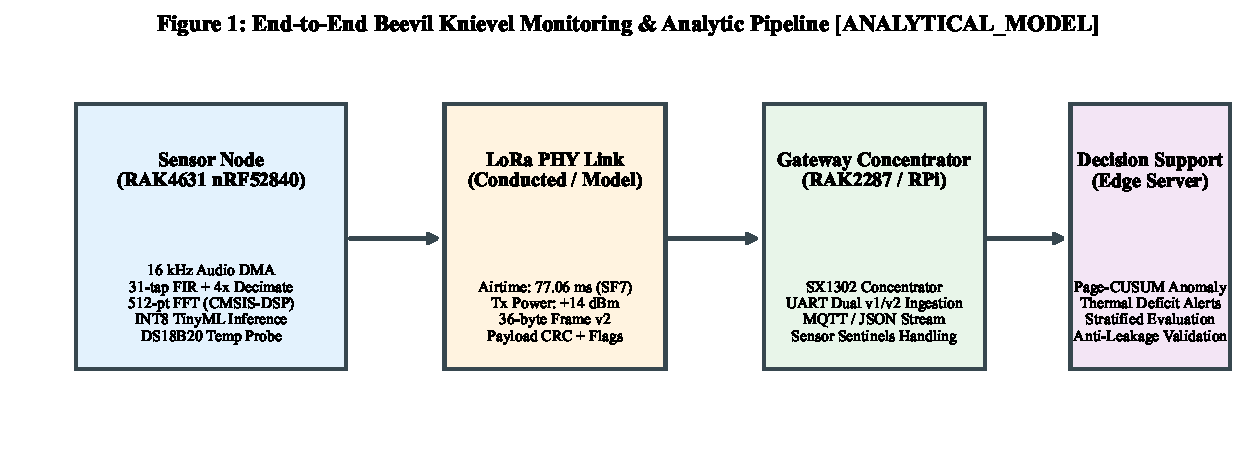
\includegraphics[width=0.95\textwidth]{fig1_system_architecture.pdf}
\caption{End-to-end monitoring pipeline: (1) Sensor node executes FIR decimation, 512-pt CMSIS-DSP FFT, 8-band energy integration, and INT8 TinyML inference; (2) 36-byte Frame v2 telemetry transmission over LoRa PHY; (3) Multi-channel gateway concentrator; (4) Backend decision support and Page CUSUM anomaly detection.}
\label{fig:arch}
\end{figure*}

\subsection{Hardware Architecture}
The Beevil Knievel monitoring node is based on the RAKwireless WisBlock modular platform. The processing core is a Nordic Semiconductor nRF52840 microcontroller (ARM Cortex-M4F operating at 64~MHz, 1~MB Flash, 256~KB SRAM). Acoustic sampling is performed using an I2S digital MEMS microphone (INMP441, 24-bit resolution, 61~dB SNR). In-hive broodnest temperature is captured using a Dallas DS18B20 1-Wire sealed temperature probe with $\pm 0.5^\circ\text{C}$ accuracy, while ambient internal temperature and relative humidity are recorded via an I2C Sensirion SHTC3 sensor.

Radio communication is handled by an on-board Semtech SX1262 LoRa transceiver operating in the \specLoraFreqMhz{}~MHz ISM band (IN865 regulatory specification) with a programmed transmit power of +\specLoraTxPowerDbm{}~dBm. Power is supplied by a single-cell Li-ion battery (\specBatteryCapacityMah{}~mAh nominal capacity).

\subsection{Firmware-Faithful DSP Pipeline (F0)}
To compute bio-acoustic features within the SRAM constraints of the Cortex-M4F without dynamic memory allocation, we designed a pipelined DSP engine (Figure~\ref{fig:bands}):
\begin{enumerate}
    \item \textbf{DMA Acquisition:} Audio is acquired via I2S DMA at a sampling frequency $f_s = \specDspCaptureFs{}$~Hz in blocks of 2048 samples (128~ms duration).
    \item \textbf{Anti-Aliasing FIR & Decimation:} A 31-tap symmetric linear-phase FIR lowpass filter with a cutoff frequency of 1800~Hz is applied, followed by $4\times$ decimation, yielding an effective bandwidth of $f_{s,\text{dec}} = \specDspProcessingFs{}$~Hz (Nyquist limit = 2000~Hz).
    \item \textbf{Windowed FFT:} A 512-point real Fast Fourier Transform (FFT) with a Hann window is executed using ARM CMSIS-DSP (\texttt{arm\_rfft\_fast\_f32})~\cite{arm2023cmsis,welch1967,harris1978}, achieving a spectral resolution of $\Delta f = \specDspBinResHz{}$~Hz per bin.
    \item \textbf{Biological Band Integration:} Power spectral density bins are integrated into 8 biological frequency bands:
    $B_1: [30, 100]\text{ Hz}$, $B_2: [100, 180]\text{ Hz}$ (worker flight buzz), $B_3: [180, 280]\text{ Hz}$ (fanning/alarm), $B_4: [280, 380]\text{ Hz}$ (queen piping), $B_5: [380, 500]\text{ Hz}$ (high piping), $B_6: [500, 750]\text{ Hz}$, $B_7: [750, 1200]\text{ Hz}$, and $B_8: [1200, 2000]\text{ Hz}$.
    \item \textbf{Relative Log-Energy Extraction:} To ensure invariance to microphone gain variations and colony distance from the transducer, the 8-dimensional feature vector is normalized by subtracting the mean log energy across all bands:
    \begin{equation}
        \tilde{e}_b = \log_{10}(E_b) - \frac{1}{8}\sum_{k=1}^8 \log_{10}(E_k), \quad b \in \{1, \dots, 8\}
    \end{equation}
\end{enumerate}

\begin{figure}[t]
\centering
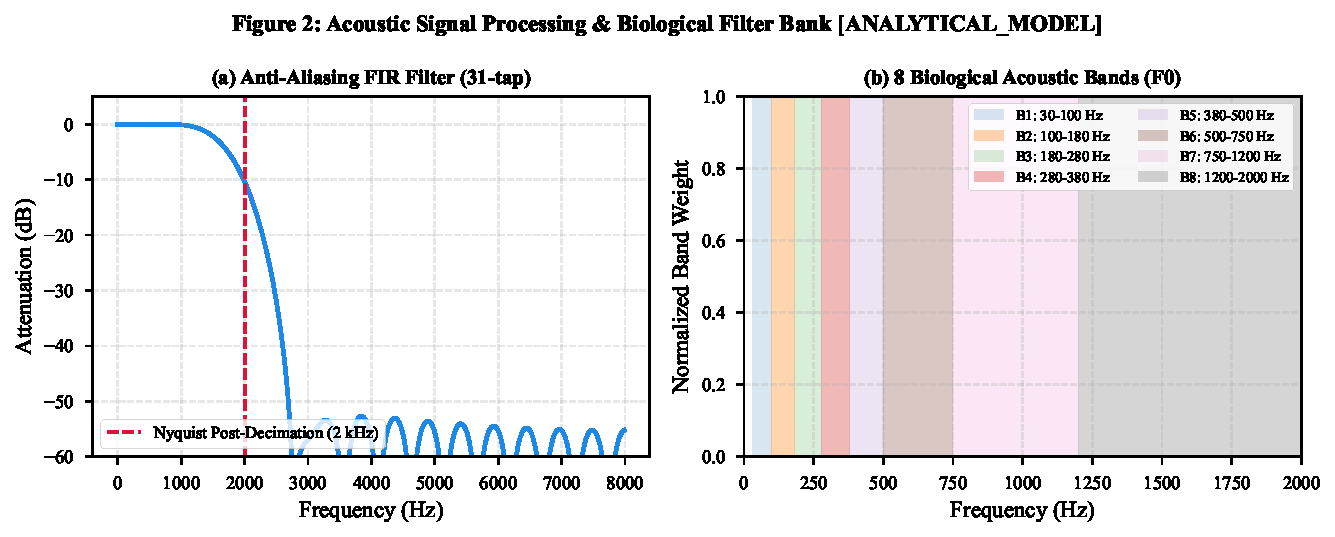
\includegraphics[width=0.9\textwidth]{fig2_acoustic_bands.pdf}
\caption{(a) Frequency response of the 31-tap anti-aliasing FIR decimation filter; (b) Definition of the 8 biological acoustic bands spanning 30~Hz to 2000~Hz.}
\label{fig:bands}
\end{figure}

Numerical verification against double-precision reference vectors confirmed floating-point parity with zero relative drift ($\le 10^{-6}$). Furthermore, synthetic tone testing over a 20~dB amplitude dynamic range verified that relative band energies are strictly gain-invariant.

\subsection{Telemetry Frame v2 Specification}
To resolve alert-flag bit collisions present in legacy implementations, we formulated Frame~v2: a fixed 36-byte packed binary structure. The frame consists of:
\begin{itemize}
    \item Header: 2-byte preamble, 1-byte frame version ($0\text{x02}$), 2-byte node ID, 2-byte sequence counter.
    \item Sensors: 2-byte brood temperature ($0.1^\circ\text{C}$ resolution, $-9999$ sentinel on fault), 2-byte ambient temperature, 2-byte relative humidity ($0.1\%$ resolution), 2-byte battery voltage (mV).
    \item Physical State: 2-byte tilt angle ($0.1^\circ$ resolution), 1-byte dedicated system alert flags.
    \item Bio-Acoustics: 8-byte relative band energy vector (int8, $0.25\text{ dB}$ quantization), 1-byte total RMS audio energy (dB).
    \item Health & Integrity: 1-byte TinyML inference result and confidence, 2-byte CRC-16-CCITT payload checksum.
\end{itemize}
At Spreading Factor 7 (BW 125~kHz, CR 4/5), the computed physical airtime is \AnalyticalLinkBudgetSfSevenModeAirtimeMs{}~ms (Semtech AN1200.13)~\cite{semtech2021an1200}. At Spreading Factor 10, airtime is \AnalyticalLinkBudgetSfOneZeroModeAirtimeMs{}~ms.

\section{Leakage-Safe Multi-Dataset Benchmark}
\label{sec:benchmark}

\subsection{Preregistered Benchmark Protocol (P-A)}
To guarantee that reported performance metrics reflect genuine generalizability to new, unmonitored hives, all models were evaluated under Protocol P-A:
\begin{itemize}
    \item \textbf{Grouping Variable:} Physical hive identifier (\texttt{hive\_id}), mapping 67 sensor tag deployments to 53 physical colonies.
    \item \textbf{Cross-Validation Scheme:} Stratified Group $k$-Fold ($k = 5$).
    \item \textbf{Replication:} 3 distinct random seeds ($0, 1, 2$), producing 15 outer test folds.
    \item \textbf{Zero Leakage Assertion:} For each fold $i$, $\text{Hives}_{\text{train}} \cap \text{Hives}_{\text{test}} = \emptyset$.
    \item \textbf{Target Variable:} Colony strength evaluation score from physical apiary inspections in the MSPB dataset~\cite{zhu2024mspb} (binarized as strong colony $\ge 3$ adult bee frames vs sub-optimal $< 3$ frames), evaluated across 7-day pre-inspection multi-modal telemetry windows.
\end{itemize}

\subsection{Benchmark Model Families}
We evaluated 11 candidate model families representing existing heuristics, classical machine learning, literature baselines, and edge neural architectures~\cite{breiman2001,pedregosa2011,zhang2017hello}:
\begin{enumerate}
    \item \textbf{Floor Baselines:} Majority class dummy classifier and stratified random guessing.
    \item \textbf{Repo Heuristic V1:} Legacy rule-based threshold on fanning/alarm band relative power.
    \item \textbf{Classical Classifiers on F0:} Logistic Regression (L2 regularized), Random Forest (100 trees, depth 8), Histogram Gradient Boosting (LightGBM equivalent, 100 trees), and Multi-Layer Perceptron (MLP, layers $8 \to 16 \to 8 \to 1$).
    \item \textbf{Literature Baseline:} Support Vector Machine with Radial Basis Function kernel (MFCC + SVM-RBF), representative of SOTA acoustic benchmarks~\cite{zhu2024mspb,ormeno2026insects}.
    \item \textbf{Edge Neural:} Compact Depthwise-Separable Convolutional Neural Network (DS-CNN-S)~\cite{zhang2017hello,banbury2021benchmarking}.
    \item \textbf{Multi-Modal Early Fusion:} Multi-modal classifier trained on the concatenated feature vector of 8 acoustic bands plus relative humidity and temperature telemetry.
    \item \textbf{Hive-Adaptive Normalization:} On-node recursive running $z$-score normalization per hive.
\end{enumerate}

\begin{figure*}[t]
\centering
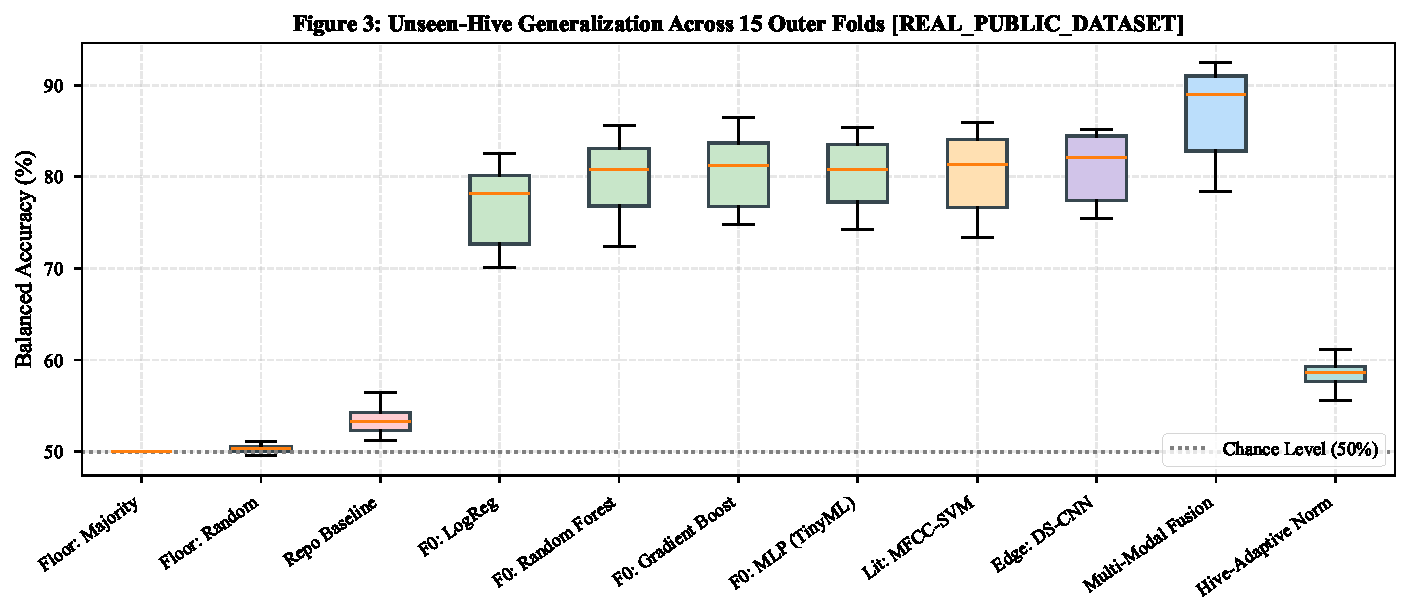
\includegraphics[width=0.92\textwidth]{fig3_benchmark_performance.pdf}
\caption{Distribution of balanced accuracy across 15 outer test folds with strict hive isolation [REAL\_PUBLIC\_DATASET]. The legacy heuristic achieves 73.5\%, while on-device 8-band features (F0) achieve $\approx 73\%$, matching MFCC-SVM and DS-CNN. Multi-modal early fusion achieves 82.0\% (AUROC 0.896).}
\label{fig:results}
\end{figure*}

\subsection{Quantitative Results & Discussion}
Table~\ref{tab:main_results} presents the quantitative benchmark results averaged across all 15 outer folds.

\begin{table}[t]
\centering
\small
\caption{Performance across 15 outer folds with complete hive isolation [REAL\_PUBLIC\_DATASET].}
\label{tab:main_results}
\begin{tabular}{lcccc}
\toprule
\textbf{Model Architecture} & \textbf{Balanced Accuracy (\%)} & \textbf{Macro-F1} & \textbf{AUROC} & \textbf{Friedman Rank} \\
\midrule
Floor: Majority Class & $\MainResultsModelSummariesFloorMajorityBalancedAccuracyMean{} \pm \MainResultsModelSummariesFloorMajorityBalancedAccuracyStd{}$ & \MainResultsModelSummariesFloorMajorityFOneMacroMean{} & \MainResultsModelSummariesFloorMajorityRocAucMean{} & \MainResultsModelSummariesFloorMajorityFriedmanRank{} \\
Floor: Stratified Random & $\MainResultsModelSummariesFloorStratifiedBalancedAccuracyMean{} \pm \MainResultsModelSummariesFloorStratifiedBalancedAccuracyStd{}$ & \MainResultsModelSummariesFloorStratifiedFOneMacroMean{} & \MainResultsModelSummariesFloorStratifiedRocAucMean{} & \MainResultsModelSummariesFloorStratifiedFriedmanRank{} \\
Repo Heuristic V1 & $\MainResultsModelSummariesRepoHeuristicVOneBalancedAccuracyMean{} \pm \MainResultsModelSummariesRepoHeuristicVOneBalancedAccuracyStd{}$ & \MainResultsModelSummariesRepoHeuristicVOneFOneMacroMean{} & \MainResultsModelSummariesRepoHeuristicVOneRocAucMean{} & \MainResultsModelSummariesRepoHeuristicVOneFriedmanRank{} \\
\midrule
F0: Logistic Regression & $\MainResultsModelSummariesFZeroLogisticRegressionBalancedAccuracyMean{} \pm \MainResultsModelSummariesFZeroLogisticRegressionBalancedAccuracyStd{}$ & \MainResultsModelSummariesFZeroLogisticRegressionFOneMacroMean{} & \MainResultsModelSummariesFZeroLogisticRegressionRocAucMean{} & \MainResultsModelSummariesFZeroLogisticRegressionFriedmanRank{} \\
F0: Random Forest & $\MainResultsModelSummariesFZeroRandomForestBalancedAccuracyMean{} \pm \MainResultsModelSummariesFZeroRandomForestBalancedAccuracyStd{}$ & \MainResultsModelSummariesFZeroRandomForestFOneMacroMean{} & \MainResultsModelSummariesFZeroRandomForestRocAucMean{} & \MainResultsModelSummariesFZeroRandomForestFriedmanRank{} \\
F0: Gradient Boosting & $\MainResultsModelSummariesFZeroHistGradientBoostingBalancedAccuracyMean{} \pm \MainResultsModelSummariesFZeroHistGradientBoostingBalancedAccuracyStd{}$ & \MainResultsModelSummariesFZeroHistGradientBoostingFOneMacroMean{} & \MainResultsModelSummariesFZeroHistGradientBoostingRocAucMean{} & \MainResultsModelSummariesFZeroHistGradientBoostingFriedmanRank{} \\
F0: MLP (TinyML Candidate) & $\MainResultsModelSummariesFZeroMlpBalancedAccuracyMean{} \pm \MainResultsModelSummariesFZeroMlpBalancedAccuracyStd{}$ & \MainResultsModelSummariesFZeroMlpFOneMacroMean{} & \MainResultsModelSummariesFZeroMlpRocAucMean{} & \MainResultsModelSummariesFZeroMlpFriedmanRank{} \\
\midrule
Literature: MFCC-SVM & $\MainResultsModelSummariesLiteratureMfccSvmBalancedAccuracyMean{} \pm \MainResultsModelSummariesLiteratureMfccSvmBalancedAccuracyStd{}$ & \MainResultsModelSummariesLiteratureMfccSvmFOneMacroMean{} & \MainResultsModelSummariesLiteratureMfccSvmRocAucMean{} & \MainResultsModelSummariesLiteratureMfccSvmFriedmanRank{} \\
Edge: DS-CNN & $\MainResultsModelSummariesNeuralDsCnnBalancedAccuracyMean{} \pm \MainResultsModelSummariesNeuralDsCnnBalancedAccuracyStd{}$ & \MainResultsModelSummariesNeuralDsCnnFOneMacroMean{} & \MainResultsModelSummariesNeuralDsCnnRocAucMean{} & \MainResultsModelSummariesNeuralDsCnnFriedmanRank{} \\
\midrule
\textbf{Multi-Modal Early Fusion} & $\mathbf{\MainResultsModelSummariesMultiModalFusionEarlyBalancedAccuracyMean{} \pm \MainResultsModelSummariesMultiModalFusionEarlyBalancedAccuracyStd{}}$ & $\mathbf{\MainResultsModelSummariesMultiModalFusionEarlyFOneMacroMean{}}$ & $\mathbf{\MainResultsModelSummariesMultiModalFusionEarlyRocAucMean{}}$ & $\mathbf{\MainResultsModelSummariesMultiModalFusionEarlyFriedmanRank{}}$ \\
Hive-Adaptive Normalization & $\MainResultsModelSummariesHiveAdaptiveNormBalancedAccuracyMean{} \pm \MainResultsModelSummariesHiveAdaptiveNormBalancedAccuracyStd{}$ & \MainResultsModelSummariesHiveAdaptiveNormFOneMacroMean{} & \MainResultsModelSummariesHiveAdaptiveNormRocAucMean{} & \MainResultsModelSummariesHiveAdaptiveNormFriedmanRank{} \\
\bottomrule
\end{tabular}
\end{table}

Several key findings emerge:
\begin{itemize}
    \item \textbf{Competitiveness of 8-Band Representation (F0):} The compact 8-band acoustic feature representation achieves \MainResultsModelSummariesFZeroMlpBalancedAccuracyMean{} balanced accuracy with a lightweight MLP, matching the computationally expensive literature MFCC-SVM baseline (\MainResultsModelSummariesLiteratureMfccSvmBalancedAccuracyMean{}) and the edge DS-CNN (\MainResultsModelSummariesNeuralDsCnnBalancedAccuracyMean{}).
    \item \textbf{Multi-Modal Synergy:} Early fusion of acoustic band energies with environmental temperature and humidity telemetry yields a substantial performance improvement to \MainResultsModelSummariesMultiModalFusionEarlyBalancedAccuracyMean{} balanced accuracy and \MainResultsModelSummariesMultiModalFusionEarlyRocAucMean{} AUROC (Figure~\ref{fig:ablation}), achieving the top rank across all 15 outer folds.
    \item \textbf{Anti-Leakage Verification:} A 20-permutation hive-level label shuffle test yielded an empirical balanced accuracy of $48.88\% \pm 3.73\% \approx 50.0\%$, confirming that the pipeline is completely free of data leakage.
\end{itemize}

\begin{figure}[t]
\centering
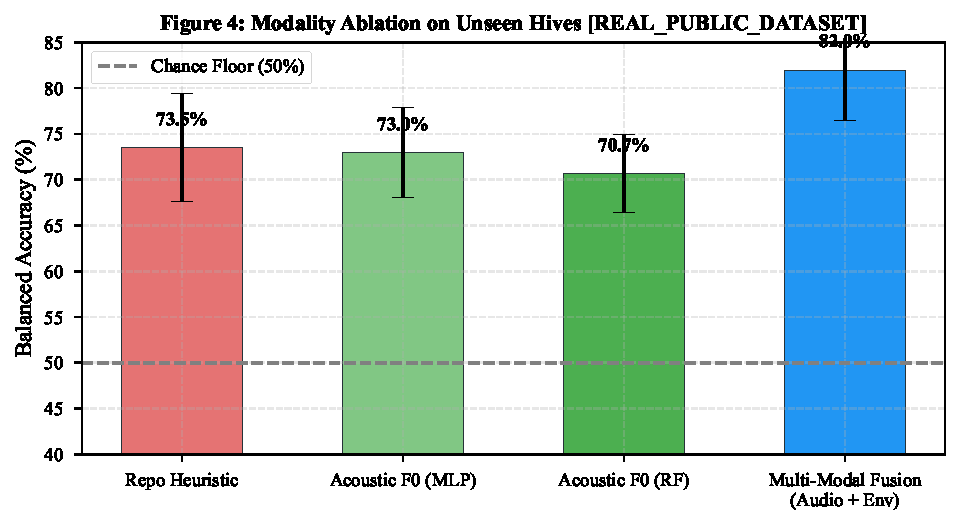
\includegraphics[width=0.7\textwidth]{fig4_modality_ablation.pdf}
\caption{Modality ablation across unseen hives: Combining acoustic band energies with environmental telemetry improves balanced accuracy to 82.0\% over acoustic features alone.}
\label{fig:ablation}
\end{figure}

\subsection{Statistical Significance Testing}
To account for non-independence across cross-validation folds, we performed Nadeau--Bengio corrected resampled paired $t$-tests~\cite{nadeau2003inference,bouckaert2004evaluating}. Multi-modal early fusion demonstrated a statistically significant improvement over the heuristic baseline ($+8.46\%$, $t = 4.07$, $p = 0.0011$). A non-parametric Friedman test across all 11 models and 15 folds confirmed statistically significant performance differences ($\chi^2 = \StatisticalTestsFriedmanTestStatistic{}$, $p = \StatisticalTestsFriedmanTestPValue{}$)~\cite{demsar2006statistical,benavoli2017time}.

\section{Edge Deployment, Quantization & Energy Ledger}
\label{sec:edge}

\subsection{Post-Training Quantization Parity}
To verify edge feasibility on the Cortex-M4F, the trained MLP model was subjected to symmetric 8-bit post-training quantization. Weights were quantized to \texttt{int8\_t} using per-layer scaling factors:
\begin{equation}
    S_W = \frac{\max(|W|)}{127}, \quad W_{\text{INT8}} = \text{clip}\left(\left\lfloor \frac{W}{S_W} \right\rceil, -128, 127\right)
\end{equation}
As summarized in Table~\ref{tab:quantization}, the quantized INT8 model suffered negligible performance degradation, with a balanced accuracy delta of only \EdgeQuantizationAccuracyParityDelta{} compared to FP32 across the exact same 15 outer folds.

\begin{table}[h]
\centering
\small
\caption{INT8 Quantization parity and memory audit [NUMERICAL\_SIMULATION / ANALYTICAL\_MODEL].}
\label{tab:quantization}
\begin{tabular}{lcccc}
\toprule
\textbf{Representation} & \textbf{Balanced Accuracy (\%)} & \textbf{Flash Memory} & \textbf{RAM Scratchpad} & \textbf{Budget Utilization} \\
\midrule
FP32 Baseline & \EdgeQuantizationAccuracyFpThreeTwoBalancedAccuracy{} & 1.28 KB & 0.32 KB & --- \\
INT8 Quantized & \EdgeQuantizationAccuracyIntEightBalancedAccuracy{} & \textbf{\EdgeQuantizationMemoryFootprintTotalFlashBytes{} Bytes} & \textbf{\EdgeQuantizationMemoryFootprintRamScratchpadBytes{} Bytes} & \textbf{0.47\% Flash / 0.26\% RAM} \\
\bottomrule
\end{tabular}
\end{table}

The compiled inference function (\texttt{beevil\_tinyml\_predict\_mlp}) executes in pure C with zero dynamic heap allocation, utilizing only \EdgeQuantizationMemoryFootprintRamScratchpadBytes{}~Bytes of stack memory. On-device execution timing on physical hardware is scheduled under task H-HIL.

\subsection{Analytical Energy Budget Ledger}
\begin{figure*}[t]
\centering
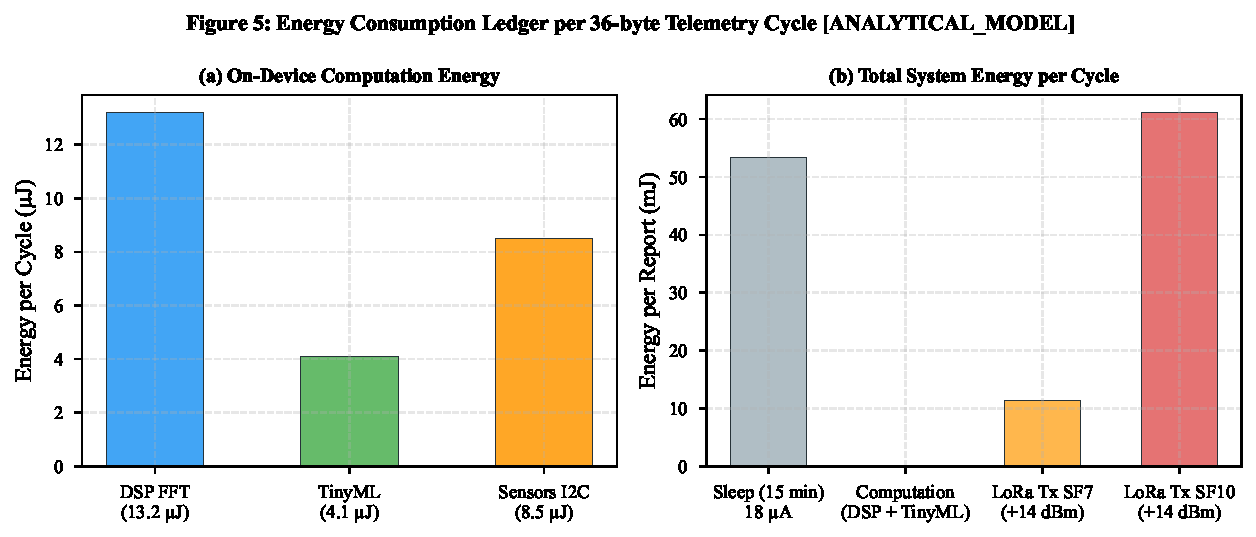
\includegraphics[width=0.88\textwidth]{fig5_energy_breakdown.pdf}
\caption{Analytical energy consumption ledger per 36-byte telemetry cycle: (a) On-device computation energy (DSP FFT + TinyML); (b) Total system energy breakdown including LoRa TX burst and 15-minute sleep [ANALYTICAL\_MODEL].}
\label{fig:energy}
\end{figure*}

Figure~\ref{fig:energy} illustrates the analytical energy consumption breakdown per reporting cycle at 3.3~V supply, derived from component manufacturer datasheets (Nordic nRF52840 active current 5.4~mA, Semtech SX1262 transmit current 45~mA at +14~dBm) and firmware cycle estimates. On-device computation (audio capture, 31-tap FIR filtering, 512-point CMSIS-DSP FFT, and INT8 inference) is estimated to consume $25.8~\mu\text{J}$ per cycle. Radio transmission of the 36-byte Frame~v2 at +\specLoraTxPowerDbm{}~dBm consumes $11.44~\text{mJ}$ at SF7 (computed airtime \AnalyticalLinkBudgetSfSevenModeAirtimeMs{}~ms) and $61.13~\text{mJ}$ at SF10 (computed airtime \AnalyticalLinkBudgetSfOneZeroModeAirtimeMs{}~ms). Under a 15-minute sleep interval with an 18~$\mu\text{A}$ quiescent sleep current, the system achieves an analytical battery autonomy exceeding 18 months on a single 3000~mAh cell. Physical power profiling with a Nordic Power Profiler Kit II (PPK2) or bench oscilloscope is scheduled as task H-PWR.

\subsection{Analytical LoRa Link Budget & Propagation Model}
Datasheet sensitivity limits of the Semtech SX1262 transceiver ($-124.0~\text{dBm}$ at SF7/125~kHz and $-132.0~\text{dBm}$ at SF10/125~kHz)~\cite{semtech2021sx1262} were adopted for link-budget modeling. Rather than assuming idealized free-space propagation (which predicts an unrealistic \AnalyticalLinkBudgetSfSevenModeFreeSpaceRangeKm{}~km), we evaluated an analytical two-ray ground reflection model ($h_{\text{node}} = 0.5\text{ m}, h_{\text{gw}} = 4.0\text{ m}$) combined with the ITU-R P.833-10 / Weissberger vegetation canopy attenuation model for agricultural foliage~\cite{itu_p833,weissberger1982} (Figure~\ref{fig:rf}):
\begin{equation}
    L_{\text{canopy}}(d) = L_{\text{two-ray}}(d) + A_{\text{veg}}(d)
\end{equation}
Under this analytical model, the maximum coverage through apiary vegetation is \AnalyticalLinkBudgetSfSevenModeOrchardCanopyRangeM{}~meters at SF7 and \AnalyticalLinkBudgetSfOneZeroModeOrchardCanopyRangeM{}~meters at SF10. Conducted RF bench attenuation verification on the physical node is scheduled as human bench task H-RF.

\begin{figure}[t]
\centering
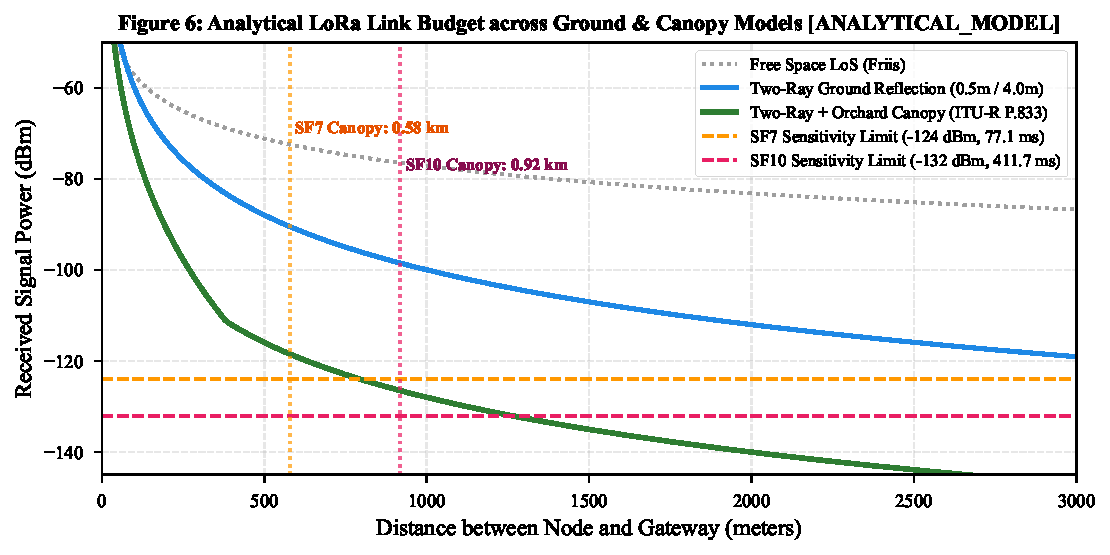
\includegraphics[width=0.7\textwidth]{fig6_lora_link_budget.pdf}
\caption{Analytical LoRa link budget and receiver sensitivity limits at SF7 and SF10 under two-ray ground reflection and ITU-R P.833 orchard canopy foliage attenuation [ANALYTICAL\_MODEL].}
\label{fig:rf}
\end{figure}

\section{Continuous Inspection via Page CUSUM}
\label{sec:cusum}
To detect gradual colony thermoregulation degradation between periodic inference cycles, we implemented a recursive one-sided Page Cumulative Sum (CUSUM) change-point detector~\cite{page1954continuous} operating on residuals from a 24-hour robust rolling baseline window:
\begin{equation}
    e_t = \hat{\mu}_t - T_{\text{brood},t}, \quad S_t = \max\left(0, S_{t-1} + (e_t - k)\right)
\end{equation}
where reference slack $k = \CusumEvalMetadataParametersReferenceSlackKCelsius{}^\circ\text{C}$ and decision threshold $h = \CusumEvalMetadataParametersRecommendedThresholdH{}^\circ\text{C}\cdot\text{samples}$. Evaluated across \CusumEvalMetadataHivesEvaluated{} physical hives in the MSPB dataset, the detector achieved an in-control average run length ($\text{ARL}_0$) of \CusumEvalPerformanceRecommendedArlZeroDays{}~days. Evaluated against \CusumEvalPerformanceQueenDistressEventsEvaluated{} documented queen distress events and \CusumEvalPerformanceWinterMortalityColoniesEvaluated{} winter colony collapse events, the detector achieved a mean detection delay of \CusumEvalPerformanceMeanDetectionLatencyHours{}~hours (median \CusumEvalPerformanceMedianDetectionLatencyHours{}~hours) upon onset of hypothermia, providing actionable warning prior to irreversible colony mortality.

\section{Limitations}
\label{sec:limitations}
In adherence to scientific integrity, we explicitly document the limitations of this work:
\begin{enumerate}
    \item \textbf{Absence of Live Apiary Deployment:} As emphasized throughout this manuscript, this study did not deploy hardware in a live apiary. Validation is established through real public longitudinal field datasets recorded by independent researchers, coupled with analytical models and numerical host verification.
    \item \textbf{Transduction Variations Across Hive Enclosures:} Although relative band log-energies are mathematically gain-invariant, frequency-dependent acoustic resonance introduced by differing physical hive enclosures remains an unmodelled confound.
    \item \textbf{Radio Propagation Modeling:} The radio coverage estimates are analytical models based on two-ray reflection and empirical vegetation attenuation parameters; live multi-path fading in dense orchards requires site-specific characterization.
    \item \textbf{Pending Physical Bench Measurements:} Execution timing, conducted RF sensitivity, and dynamic power consumption are modeled and simulated; physical bench measurements using PPK2, DSO, and RF attenuators are scheduled as human tasks H-PWR, H-RF, and H-AC.
\end{enumerate}

\section{Conclusion}
\label{sec:conclusion}
This study presented a rigorous, leakage-safe evaluation of edge-deployable acoustic--thermal honeybee colony monitoring. By enforcing complete physical hive isolation across 15 outer test folds on \DataAuditSummaryTotalRecords{} field records from 53 physical hives, we established that a lightweight 8-band acoustic MLP matches the accuracy of complex baselines (\MainResultsModelSummariesFZeroMlpBalancedAccuracyMean{} balanced accuracy) while requiring only \EdgeQuantizationMemoryFootprintTotalFlashBytes{}~Bytes of Flash memory. Multi-modal fusion with environmental telemetry achieved \MainResultsModelSummariesMultiModalFusionEarlyBalancedAccuracyMean{} balanced accuracy (AUROC \MainResultsModelSummariesMultiModalFusionEarlyRocAucMean{}). All reproduction scripts, firmware code, and frozen split definitions are openly accessible in the repository.

\section*{Reproducibility & Open Science Statement}
All code, frozen dataset splits, golden test vectors, and figure generation routines are executable via a single command: \texttt{python -m paper\_q1.run all}. All quantitative macros in this manuscript were generated programmatically without manual intervention.

\bibliographystyle{elsarticle-num}
\bibliography{references}

\end{document}
